\section{Subsidiando el transporte}

\subsection{Descripción del problema}
En este problema, observamos la provincia de Optilandia, cuyas ciudades estan conectadas por rutas de una sola dirección, donde no necesariamente se puede llegar de una ciudad a todas las demás. Sin embargo, sabemos que desde cualquier ciudad se puede llegar, al menos, a otra ciudad. Cada una de estas rutas tiene una cabina de peaje y, por ende, recorrer cada una de ellas tiene un costo. Sin embargo, por decisiones gubernamentales, cada uno de estos peajes se vio reducido por un costo fijo c (si antes la ruta A valía A1, y la ruta B valía B1, ahora valen A1 - c y B1 - c respectivamente), pudiendo generar que una ruta no solo no le cobre a sus usuarios, sino que acabe dándole dinero.

Si bien esto no es un problema para el gobierno, siempre y cuando se evite que un usuario pueda irse desde una ciudad, hacer un recorrido y volver a la misma habiendo ganado plata. Por lo tanto, como el gobierno busca maximizar el subsidio otorgado, debemos buscar el valor c que permita otorgar el mayor subsidio por peaje sin que exista la posibilidad de que un usuario le saque plata al Estado. La complejidad del algoritmo debe ser no peor que \textbf{O($nm.log(c)$)}, donde n es la cantidad de ciudades, m es la cantidad de rutas y c es el costo del máximo peaje.

Veamos un ejemplo del problema. Supongamos que tuvieramos 6 ciudades, con las siguientes rutas iniciales y con los siguientes costos de peaje1 expresados en pesos:

\bigskip

\begin{minipage}{0.5\textwidth}
	\begin{itemize}
		\item Ruta de 1 a 2. Costo de peaje: 40 pesos.

		\item Ruta de 2 a 3. Costo de peaje: 20 pesos.

		\item Ruta de 3 a 4. Costo de peaje: 10 pesos.

		\item Ruta de 4 a 1. Costo de peaje: 15 pesos.

		\item Ruta de 5 a 2. Costo de peaje: 5 pesos.

		\item Ruta de 6 a 3. Costo de peaje: 10 pesos.
	\end{itemize}
\end{minipage}
\hfill
\begin{minipage}{0.45\textwidth}

	\begin{tikzpicture}[->, >=latex]
		\begin{scope}[nodeList]
			\node (1) at (0, 0) {1};
			\node (2) at (3, 0) {2};
			\node (3) at (3, 3) {3};
			\node (4) at (0, 3) {4};
			\node (5) at (6, 0) {5};
			\node (6) at (6, 3) {6};
		\end{scope}

		\begin{scope}[pathList]
			\draw (1) -- (2) node {40};
			\draw (2) -- (3) node {20};
			\draw (3) -- (4) node {10};
			\draw (4) -- (1) node {15};
			\draw (5) -- (2) node {5};
			\draw (6) -- (3) node {10};
		\end{scope}
	\end{tikzpicture}
	
%	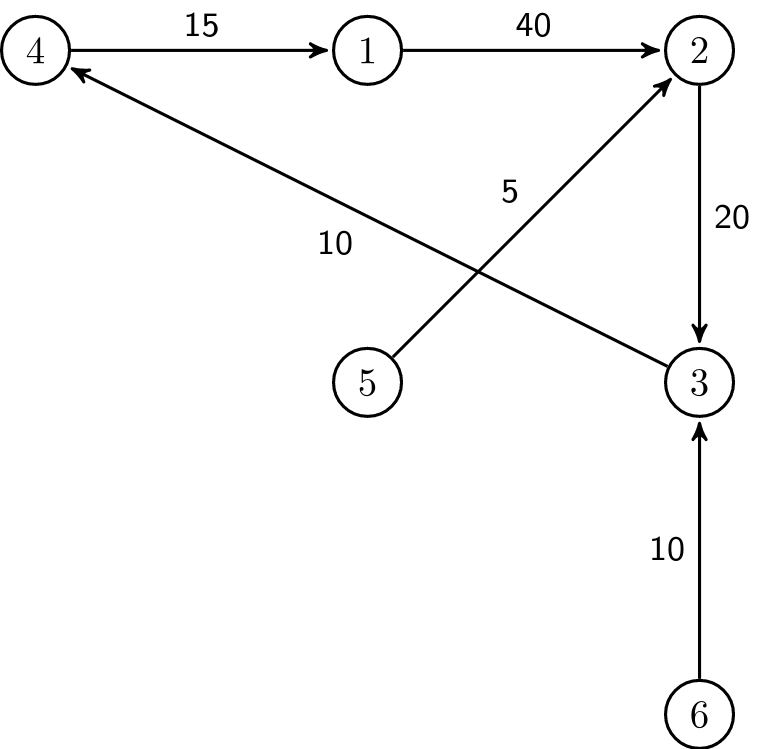
\includegraphics[scale=0.15]{imagenes/ejemplo2.png}

\end{minipage}

\bigskip

Como vemos, la única manera de salir de una ciudad y volver a la misma es que arranquemos en las ciudades 1, 2, 3 ó 4, y recorramos las cuatro rutas que las conectan. Por ende, debemos asegurar que al recorrerlas no se le saca plata al estado; es decir, que al aplicarle el subsidio fijo, se descuenta menos de (40+20+10+15) $=$ 85 pesos. Considerando que las cuatro rutas tienen el mismo descuento, el mayor subsidio que se podría realizar es la cuarta parte de 85, que si lo redondeamos es 21 pesos. Por lo tanto, el mayor descuento que se podría realizar a las rutas de esta provincia es de 21 pesos.

\subsection{Desarrollo}
Dado este problema, y considerando que hay que tener en cuenta la mano en la cual corren las rutas, la mejor manera de modelarlo sería utilizando digrafos. Así, cada ciudad se representaría con un nodo, y cada una de las rutas que conecta dos ciudades, con una arista dirigida. Consideraremos que un recorrido abusivo es representado por un ciclo negativo en el digrafo.

Como nuestro problema principal es averiguar cual es el mayor subsidio que se le puede otorgar a todas las rutas sin que se generen ciclos de rutas negativos, no es dificil que rápidamente encontremos una visión certera de lo que debemos hacer en el problema. Como primer aproximamiento, podemos asegurar que nuestro objetivo será reducir el costo de las rutas de manera que vayamos obteniendo mejores valores hasta que, superado el valor máximo, encontremos ciclos negativos en nuestro grafo.

Por ende, sabemos de entrada que necesitaremos un algoritmo capaz de reconocer ciclos negativos; y considerando los límites de complejidad brindados, concluímos que Bellman-Ford cumple nuestros propositos. Este algoritmo nos permitirá utilizar aristas negativas, y averiguar en cada uno de los nodos si en sus componentes hay o no ciclos negativos.

Dado que en el problema original queremos detectar la existencia de ciclos negativos para distintas versiones del mismo grafo, usamos una función que permite crear una nueva versión del grafo a partir del original. Diremos que una p-versión nueva del grafo contiene la misma cantidad de nodos y representa al mismo conjunto de adyacencias, y su diferencia radica en que para todo eje de u a v con peso w perteneciente al grafo original, hay un eje de u a v con peso (w-p) perteneciente a la p-versión. Así, utilizaremos un algoritmo que, para cada versión, nos diga si efectivamente al aplicarle Bellman-Ford se encuentran o no ciclos negativos (para esto, utilizamos una versión del algoritmo que nos devuelve $true$ si encuentra ciclos negativos, y $false$ si no lo hace)

Del mismo modo, dado que Bellman-Ford parte de un nodo \textit{s} y actualiza las distancias entre \textit{s} y el resto de los nodos, solo puede detectar ciclos negativos si estos pertenecen a la misma componente conexa que \textit{s}. Si el grafo G de entrada no es conexo, no existe nodo de partida que sirva para reconocer a todas las componentes de G. Por ende, proponemos la creación de un nodo con $d_{out} = n \land d_{in} = 0$. En otras palabras, para todo nodo \textit{v} perteneciente a G, existe un eje que va de \textit{s} a \textit{v}. Sin embargo, para que el mismo no afecte el resultado final, deberemos agregarlo luego de realizar la p-versión del grafo original (es decir que, sea cual sea la p-versión, las aristas que conecten a \textit{s} con cualquier otro nodo tendrán peso nulo)

A partir de esto, el algoritmo de Bellman-Ford puede utilizar a \textit{s} como nodo de partida y tendremos garantizado que reconoceremos todos los ciclos negativos del grafo. De este modo, en un grafo con \textit{n} nodos y \textit{m} aristas, pasaríamos a tener \textit{n+1} y \textit{m+n} aristas.

\begin{algorithm}[H]
	\NoCaptionOfAlgo
	\caption{\algoritmo{ajusteParaBellmanFord}{\In{p}{int}, \In{ejesGrafo}{lista[ejes]}, \In{tamano}{int}}{bool}}
	
	lista[ejes] ejesPVersion $\leftarrow$ ajustarEjes(ejesGrafo, p)
	
	lista[ejes] ejesPVersion $\leftarrow$ agregarEjeGeneral(ejesPVersion, tamaño)

	res $\leftarrow$ bellmanFord(ejesPVersion, tamaño+1)
\end{algorithm}

Es importante aclarar que, al pasarle como parámetro \textit{(tamaño+1)} a Bellman-Ford, estamos enviando el nodo de origen desde el cual se correrá el algoritmo (el cual es, justamente, el último nodo que colocamos nosotros)

Diremos que c es el peso de la arista mas pesada del grafo original. Veamos que la versión p $=$ 0 es equivalente al grafo original, y por ende no puede tener ciclos negativos. Por otro lado, veamos que si el grafo original tiene ciclos, la versión p $=$ c + 1 tendrá ciclos negativos, porque todas sus aristas serán negativas. Por ende, sabemos que nuestra solución esta acotada inferiormente por 0 y superiormente por c.

Por otro lado, teniendo en cuenta un Q cualquiera, sabemos que si la versión Q carece de ciclos negativos entonces toda versión con un valor de subsidio menor a Q también carecerá de ellos. La intuición aquí reside en notar que aumentar los pesos de un grafo sin ciclos negativos producirá el aumento del peso de todos sus ciclos, y por lo tanto, que todos ellos continuen sin ser negativos. Del mismo modo, podemos notar lo inverso: si la versión Q posee ciclos negativos, toda versión con un valor de subsidio mayor a Q los contendrá.

Entonces, sabiendo que un valor Q bien nos habla de todos los mayores o menores a él; y considerando que nuestra solución se encuentra entre 0 y c, podemos realizar una búsqueda binaria tal que para cada versión Q, si la misma posee ciclos negativos, nuestra solución se acotará entre 0 y Q. En cambio, si no los posee, su solución se encontrará entre Q y c.

Por lo tanto, con lo ya expuesto, podemos utilizar el algoritmo con ajuste de Bellman-Ford que expusimos anteriormente para averiguar cual es el máximo subsidio realizable, aplicando una suerte de búsqueda binaria sobre los valores.

\begin{algorithm}[H]
	\NoCaptionOfAlgo
	\caption{\algoritmo{subsidioDeRutas}{\In{n}{nat}, \In{ejesGrafo}{lista[ejes]}}{nat}}		
		nat: cotaInferior $\leftarrow$ 0
		
		nat: cotaSuperior $\leftarrow$ pesoMax(ejesGrafo)
		
		\While{cotaInferior $<$ cotaSuperior}{
		nat: nuevaCota $\leftarrow$ (cotaInferior + cotaSuperior) / 2
		
		bool: tieneCiclos $\leftarrow$ ajusteBellmanFord(ejesGrafo, nuevaCota)
		
		\eIf{tieneCiclos}{
			cotaSuperior $\leftarrow$ nuevaCota
			}{
			cotaInferior $\leftarrow$ nuevaCota
			}
 		}
 		res $\leftarrow$ cotaInferior
\end{algorithm}

\subsection{Cota temporal}
Luego del análisis realizado, y viendo el algoritmo subsidioDeRutas dado para el problema, el conjunto de operaciones significativas para deducir la complejidad se reduce al \textit{while} en el cual, con la ayuda del Bellman-Ford con ajuste, acabamos obteniendo el mayor subsidio posible.

Analicemos, entonces, esta porción del algoritmo. Buscamos un valor entre 0 y c, como habíamos dicho inicialmente, y cada vez que se corre el ciclo reducimos esta búsqueda a la mitad de los valores (0 y Q, o bien Q y c). Por ende, tenemos un \textit{while} que corre en $O(log(c))$, dándonos como resultado final $O(log(c).BF))$ donde BF es la complejidad del Bellman-Ford con ajuste.

Pasemos a analizar este otro algoritmo. El Bellman-Ford con ajuste realiza 3 operaciones: reajusta el valor de todos los ejes, agrega un nodo con \textit{n} ejes de peso nulo y finalmente corre Bellman-Ford desde este nodo agregado. Es facil ver que las primeras dos operaciones se reducen a recorrer todos los ejes y todos los nodos, respectivamente, y por ende corren en $O(m)$ y $O(n)$; mientras que el algoritmo de Bellman-Ford, si bien tiene complejidad $O(n.m)$ conocida, se puede ver afectada al agregar un nodo de grado \textit{n} a nuestro grafo, por lo que se requiere un análisis más exhaustivo.

Veamos lo que ocurre con nodos y aristas respectivamente. Al tener \textit{n} nodos y \textit{m} aristas, y agregar un nuevo nodo con \textit{n} aristas nuevas, pasamos a tener \textit{n+1} nodos y \textit{m+n} aristas. Por ende, si repasamos las complejidades obtenidas con estos valores, el Bellman-Ford con ajuste tendrá una cota temporal de $O(m) + O(n) + O((n+1)(m+n))$ $\subseteq$ $O(n(m+n))$ $\subseteq$ $O(n^2 + n.m)$.

Sin embargo, tenemos como premisa que todo nodo perteneciente al grafo debe tener grado de salida mayor o igual a 1 ($d_{out}$ $\geq$ $1$). Por lo tanto, por cada nodo del grafo original tenemos al menos una arista, y podemos acotar $m \geq n$. De este modo, podemos asegurar las siguientes relaciones: $O(n)$ $\subseteq$ $O(m)$ $\rightarrow$ $O(n^2)$ $\subseteq$ $O(n.m)$.

Por lo tanto, si $O(n^2)$ $\subseteq$ $O(n.m)$, podemos reducir la complejidad del Bellman-Ford con ajuste de $O(n^2 + n.m)$ a $O(n.m + n.m)$ que es exactamente $O(n.m)$. De este modo, demostramos que agregar el nodo con n aristas en el contexto de este problema no afecta la complejidad del algoritmo de Bellman-Ford.

Entonces, como habíamos dicho anteriormente, la complejidad de nuestro problema se reduce a $O(log(c).BF))$ donde BF es la complejidad del Bellman-Ford con ajuste. Y como vimos, la complejidad de este último algoritmo es de $O(n.m)$, por lo que nuestra cota temporal es finalmente $O(log(c).n.m)$, que cumple las condiciones de cota temporal exigidas por el ejercicio.

\subsection{Experimentacion}

La experimentación de este ejercicio representó un desafío, ya que en la generación de grafos resultó difícil garantizar condiciones que diesen resultados homogéneos debido a nuestra implementación. Esto requeriría crear grafos fuertemente conexos, de modo que ningún eje estuviese fuera de un ciclo. Sin embargo, sí pudimos observar fácilmente los casos de grafos completos.

\begin{center}
	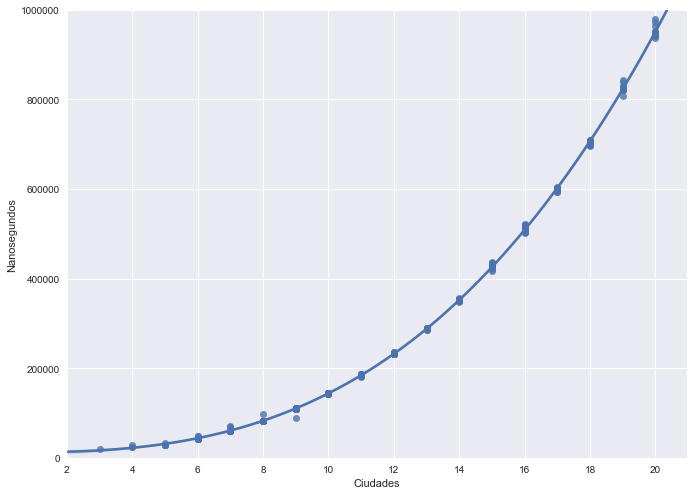
\includegraphics[scale=0.5]{imagenes/ej2-1.png}
\end{center}

En este gráfico se puede observar que, en grafos completos, el algorítmo tiene complejidad cúbica con respecto a la cantidad de ciudades. Esto se ajusta a la complejidad pedida, ya que $m = \frac{n \times (n-1)}{2} \approx n^2$, es decir, $O(n m) \subseteq O(n^3)$.

\begin{center}
	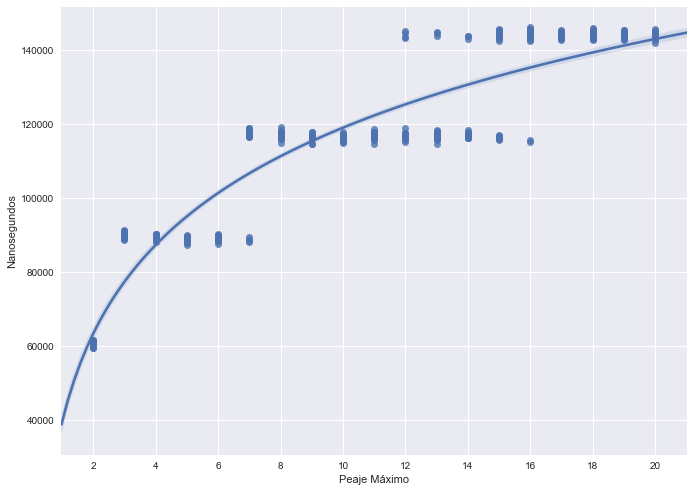
\includegraphics[scale=0.5]{imagenes/ej2-2.png}
\end{center}

Por otro lado, podemos ver que el máximo peaje tiene impacto logarítmico sobre el tiempo de ejecución, lo que condice con nuestras expectativas y con la cota de complejidad pedida.
